\chapter{Normalisasi Teks dengan Jarak Levenshtein}

\section{Alur Proses Normalisasi Teks dengan Jarak Levenshtein}

Gambar \ref{fig:side_to_side} bagian (a) menunjukkan alur proses untuk rancangan metode normalisasi yang diusulkan. Metode normalisasi usulan menggunakan jarak Levenshtein sebagai penghitungan jarak antara kedua teks. Deskripsi alur proses yang dijalankan dapat dijelaskan sebagai berikut:
\begin{enumerate}
	\item diberikan kata masukan dan kamus kata baku,
	\item melakukan pencarian kata-kata dalam kamus kata baku yang memiliki jarak minimum dengan kata masukan menggunakan jarak Levenshtein, menghasilkan kumpulan kata, dan,
	\item melakukan seleksi kata yang menjadi kata keluaran. Jika terdapat lebih dari satu kata, maka kata yang dipilih adalah kata yang pertama kali ditemukan.
\end{enumerate}
\begin{figure}[ht]
	\centering
	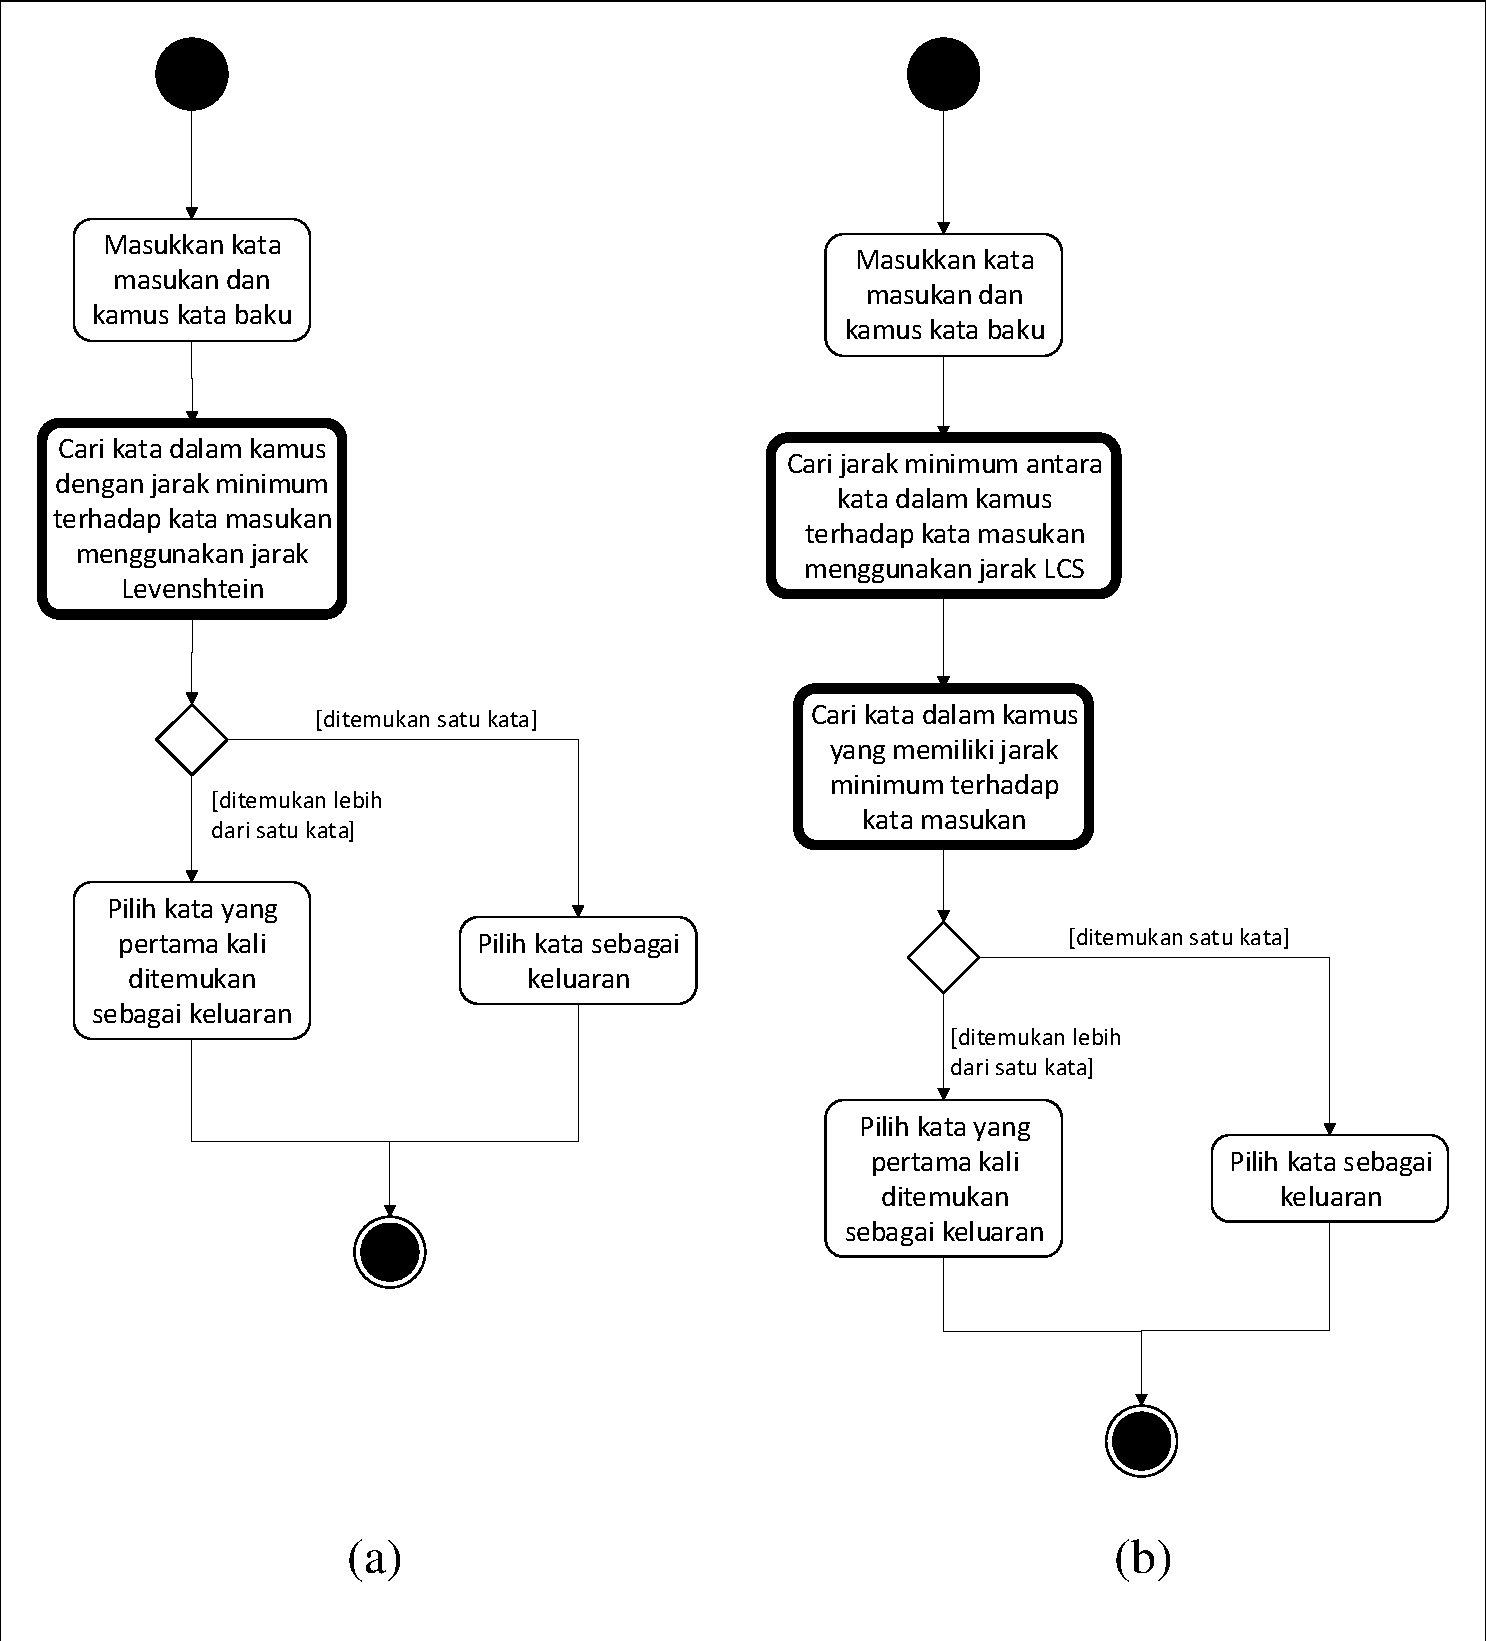
\includegraphics[width=0.8\textwidth, trim=2 2 2 2, clip]{resources/3/side_to_side.pdf}
	\caption{Alur proses normalisasi teks dengan (a) jarak Levenshtein, dan (b) jarak LCS \parencite{saragih2017normalisasi}}
	\label{fig:side_to_side}
\end{figure}

Terdapat perbedaan alur proses antara metode normalisasi \parencite{saragih2017normalisasi} dengan metode normalisasi menggunakan jarak Levenshtein. Perbedaan tersebut dapat dilihat pada blok proses dengan garis tepi tebal pada Gambar \ref{fig:side_to_side}. Perbedaan pertama terletak pada penggantian algoritme jarak LCS dengan jarak Levenshtein. Kedua, metode normalisasi usulan mempersingkat proses normalisasi dengan menemukan kumpulan kata prediksi dengan jarak minimum secara langsung dibandingkan metode normalisasi \parencite{saragih2017normalisasi} yang harus mencari jarak minimum terlebih dahulu kemudian menemukan kumpulan kata prediksi dengan jarak tersebut.

\section{Algoritme Normalisasi Teks dengan Jarak Levenshtein}

Algoritme \ref{lst:lv} merupakan algoritme persamaan jarak Levenshtein yang dapat dilihat pada Rumus \ref{eq:lv} \parencite{levenshtein1966binary}. Algoritme menerima masukan berupa dua kata dan mengeluarkan nilai jarak perubahan berupa bilangan bulat. Penghitungan jarak perubahan kedua kata masukan dilakukan dengan menggunakan matriks dua dimensi dengan ukuran matriks disesuaikan dengan kedua masukan kata tersebut.
\begin{lstlisting}[caption={Algoritme Fungsi Jarak Levenshtein},label={lst:lv},float,floatplacement=H]
Masukan: str1, str2		: string
Keluaran: integer

Deklarasi:
str1, str2 				: string
len1, len2, i, j, actv 	: integer
matrix					: array[][] integer

Deskripsi:
Mulai
1. Menambah str1 dan str2 dengan spasi di depan;
2. masukkan secara berurutan nilai panjang str1 dan str2 ke dalam variabel len1 dan len2;
3. membuat matrix dengan ukuran len1 x len2 lalu isi semua sel dengan nilai 0;
4. selama i diantara 1 dan len1 - 1, isi sel matrix[i][0] dengan nilai i;
5. selama j diantara 1 dan len2 - 1, isi sel matrix[0][j] dengan nilai j;
6. selama i diantara 1 dan len1 - 1 dan j diantara 1 dan len2 - 1:
	a) masukkan variabel actv dengan nilai 1;
	b) jika str1[i] sama dengan str2[j], ubah nilai actv dengan nilai 0;
	c) masukkan variabel matrix[i][j] dengan nilai terkecil antara matrix[i-1][j] + 1, matrix[i][j-1] + 1, atau matrix[i-1][j-1] + actv.
7. keluarkan nilai dalam variabel matrix[len1-1][len2-1].
Selesai
\end{lstlisting}

Fungsi dalam Algoritme \ref{lst:lv} digunakan untuk metode normalisasi kata pada Algoritme \ref{lst:lev_find} dengan tujuan untuk mencari kumpulan kata yang memiliki jarak perubahan paling kecil. Terdapat dua masukan metode yaitu sebuah kata dan sebuah kamus dalam bentuk vektor. Metode menghasilkan dua keluaran, yaitu nilai jarak terkecil antara kata masukan dengan seluruh kata dalam kamus dan vektor berisi kumpulan kata dengan jarak terkecil dengan kata masukan.
\begin{lstlisting}[caption={Algoritme Fungsi Normalisasi Kata dengan Jarak Levenshtein},label={lst:lev_find},float,floatplacement=h]
Masukan: txt : string, kam : dictionary
Keluaran: array, integer

Deklarasi:
txt, word		: string
val, minVal 	: integer
kam				: dictionary
similarWords	: array[] string

Deskripsi:
Mulai
1. Masukkan nilai 30 ke dalam variabel minVal;
2. masukkan nilai txt ke dalam vektor similarWords;
3. untuk seluruh kata dalam kam:
	a) Masukkan nilai kata ke dalam variabel word;
	b) hitung jarak Levenshtein antara txt dengan word, simpan hasil ke dalam variabel val;
	c) jika val lebih kecil dari minVal:
		i) jika val sama dengan nol (0), jadikan word sebagai vektor lalu keluarkan vektor bersama dengan nilai 0;
		ii) jika val tidak sama dengan nol, ganti similarWords dengan vektor berisi word lalu ganti minVal dengan val.
	d) jika val sama dengan minVal, tambah nilai ke dalam array similarWords.
4. keluarkan array similarWords dan nilai dalam variabel minVal.
Selesai
\end{lstlisting}

Berbagai kondisional yang tercantum dalam Algoritme \ref{lst:lev_find} dijelaskan sebagai berikut:
\begin{enumerate}
	\item "jika \textit{val} sama dengan nol (0)" yaitu kata masukan (\textit{txt}) dan kata dalam kamus (\textit{word}) adalah kata yang sama persis, ditunjukkan dengan jarak perubahan (\textit{val}) bernilai nol. Oleh karena itu, \textit{word} langsung diubah menjadi vektor lalu dijadikan sebagai keluaran fungsi beserta nilai jaraknya yaitu nol;
	\item "jika \textit{val} tidak sama dengan nol" yaitu ditemukan \textit{word} dengan jarak yang lebih kecil dibandingkan jarak terkecil (\textit{minVal}) sebelumnya sehingga seluruh isi vektor kumpulan kata (\textit{similarWords}) terdahulu harus dibuang lalu digantikan dengan \textit{word}; dan
	\item "jika \textit{val} sama dengan \textit{minVal}" yaitu ditemukan \textit{word} yang memiliki jarak yang sama dengan seluruh kata dalam \textit{similarWords} sehingga \textit{word} harus dimasukkan ke dalam \textit{similarWords}.
\end{enumerate}

\section{Contoh Normalisasi Teks dengan Jarak Levenshtein}

Contoh normalisasi teks dengan jarak Levenshtein tertera pada Tabel \ref{tbl:eg_output}. Salah satu contoh yang digunakan adalah kata "\textit{mikir}". Kata "\textit{mikir}" memiliki keluaran kumpulan kata-kata baku, yaitu "pikir", "bikir", "kikir", "likir", "milir", dan "zikir". Semua kata baku tersebut memiliki jarak perubahan yang sama dengan kata "\textit{mikir}" yaitu 1. Jarak tersebut juga merupakan jarak terkecil yang dapat dicapai antara kata masukan dengan seluruh kata yang ada di dalam kamus.
\begin{table}[ht]
    \captionsetup{justification=justified,singlelinecheck=false}
    \caption{Contoh keluaran Normalisasi Teks dengan Jarak Levenshtein}
    \label{tbl:eg_output}
    \centering
    \begin{tabularx}{\textwidth}{|Y|X|X|}
        \hline
        \textbf{Contoh kata masukan} & \multicolumn{1}{Y|}{\textbf{Contoh keluaran kumpulan kata}} & \multicolumn{1}{Y|}{\textbf{Contoh keluaran jarak terkecil}} \\ \hline
        \textit{mikir} & {[}'pikir', 'bikir', 'kikir', 'likir', 'milir', 'zikir'] & 1 \\ \hline
        \textit{maen} & {[}'main', 'man', 'men'] & 1 \\ \hline
        \textit{begimana} & {[}'bagaimana', 'begana']& 2 \\ \hline
    \end{tabularx}
\end{table}